\section{Introduction}
\label{sec:introduction}


The discovery of a new particle in 2012~\cite{Aad:2012tfa,Chatrchyan:2012xdj,Chatrchyan:2013lba}, widely believed to be the Higgs boson, at the Large Hadron Collider was a milestone in the history of particle physics.
% 
The Higgs boson, predicted independently and roughly simultaneously in Refs.~\cite{Higgs:1964pj,Englert:1964et,Guralnik:1964eu}, solved the long-standing puzzle of the heavy $\zboson$ and $\wboson$ bosons, and could explain the mechanism behind the mass generation of fermions as well.
% 
Since then, a wealth of data has been collected by the LHC experiments, notably the CMS and ATLAS experiments, in an effort to further narrow down the properties of the Higgs boson and to improve our understanding of electroweak symmetry breaking.


As ever more experimental evidence suggests that the properties of the newly discovered particle are in fact consistent with those of the standard model Higgs boson,
% 
% As the basic properties of the newly discovered particle, such as the final states to which it decays, are more and more consistent with the standard model Higgs boson,
% 
the study of the Higgs boson becomes increasingly a matter of \textit{precision}: To what extent does the particle behave like the standard model Higgs boson, exactly?
% 
And importantly, at what point will the standard model significantly deviate from observations?
% 
With around 300\fbinv of data collected by the end of 2023, and much more to be collected in the future~\cite{hllhc}, the study of the Higgs boson enters a precision era, in which the standard model is tested in ever more clever ways to either confirm it, or to prove that there must be more, new physics.


So far, however, the standard model has proven to very resilient---almost frustratingly so, if one hopes to observe physics beyond the standard model in order to explain some of its theoretical and experimental gaps.
% 
A promising way of hunting for deviations to the standard model, which may point to new physics, is provided by measurements of the Higgs boson couplings to other particles.
% 
Notable models of new physics that modify the coupling of the Higgs boson include, for example, supersymmetry~\cite{Dimopoulos:1981zb,Witten:1981nf}, or heavy top partners~\cite{ArkaniHamed:2002qy,Banfi:2013yoa}.
% 
The latest precision measurement from the CMS Collaboration~\cite{Sirunyan:2018koj}, a combination of many Higgs boson decay channels, reveals no deviations from the standard model so far.
% 
Figure~\ref{fig:productiondecay} shows the measured Higgs boson couplings based on inclusive cross section measurements; the agreement with the standard model is striking.
% 
Other inclusive cross section measurements~\cite{Khachatryan:2016vau,Aad:2015zhl} yield a similar picture.


\begin{figure}[hbtp]
  \begin{center}
    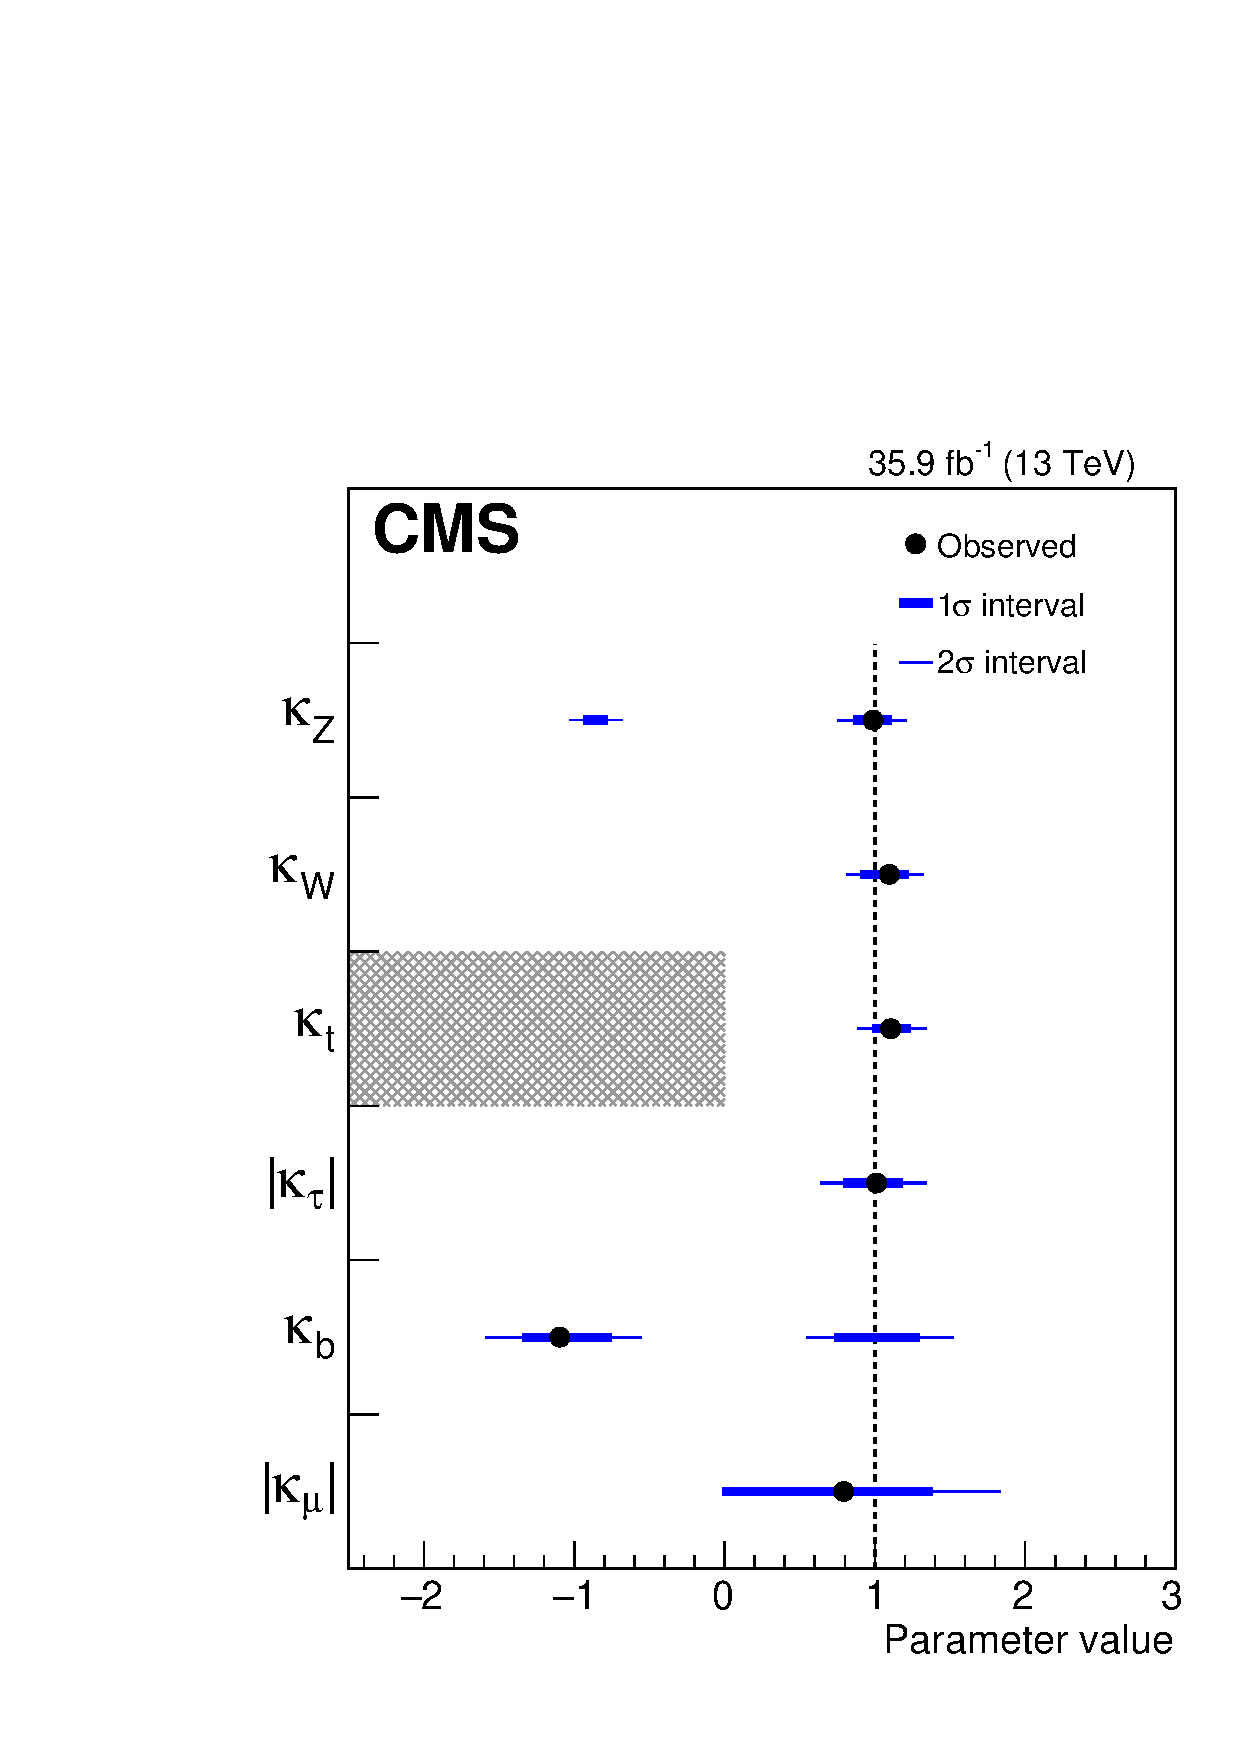
\includegraphics[width=\halflinewidth]{img/cmscombcouplings.pdf}
    \caption{%
        Measurements of the Higgs boson couplings to other particles from the CMS detector~\cite{Sirunyan:2018koj}, using data collected at $\sqrt{s}=13$\TeV corresponding to an integrated luminosity of $36.1$\fbinv.
        % 
        The dashed black line indicates the standard model expectation.
        % 
        The underlying model of this fit result assumes no beyond-the-standard-model physics.
        % 
        Taken from Ref.~\cite{Sirunyan:2018koj}.
        }
    \label{fig:productiondecay}
  \end{center}
\end{figure}


The advent of more data will surely improve the precision of the picture provided by Fig.~\ref{fig:productiondecay}.
% 
Presently, however, it is of interest to move beyond inclusive cross section measurements, and to see to what extent the standard model holds in more involved measurements.
% 
A promising avenue is the use of differential cross sections~\cite{Aad:2014lwa,Khachatryan:2015rxa,Aad:2014tca,Khachatryan:2015yvw,Aad:2016lvc,Khachatryan:2016vnn,Aaboud:2018xdt,Sirunyan:2018kta,Aaboud:2017oem,Sirunyan:2017exp,Aaboud:2018ezd}, which concern cross section measurements as a function of a kinematic variable, such as the transverse momentum $\pt$.
% 
Compared to inclusive cross section measurements, differential cross section measurements allow the exploration of deviations from the standard model in particular regions of phase space, that would not be observed in inclusive cross section measurements.
% 
A notable example is the modification of the Higgs boson coupling to the top quark, which manifests as deviations in the differential cross section at large $\pt$~\cite{Grazzini:2017szg,Grazzini:2016paz}; since the cross section in this region of phase space is a mere fraction of the cross section at low $\pt$, this effect is hard to observe in an inclusive cross section measurement.


After a treatment of the theoretical and practical fundamentals of high energy physics, this thesis concerns first a combination of differential cross section measurements in order to obtain the most precise differential spectra as possible.
% 
Inputs to the combination include differential cross section measurements made in the Higgs-to-diphoton~\cite{Sirunyan:2018kta} and Higgs-to-four-leptons~\cite{Sirunyan:2017exp} decay channels, using data recorded by the CMS experiment in 2016 at $\sqrt{s}=13$\TeV corresponding to an integrated luminosity of $35.9\fbinv$.
% 
The kinematics of the Higgs boson are fully described by the Higgs boson mass $\mh$, the rapidity $\absy$, and its transverse momentum $\pth$, and as such the spectra are naturally combined for the variables $\absy$ and $\pth$.
% 
In order to improve the precision at large $\pt$, a search for the Higgs boson produced with a large $\pt$ and decaying to a bottom quark-antiquark pair~\cite{Sirunyan:2017dgc} is included for the combination of the $\pt$ spectrum.
% 
% The $\absy$ distribution is determined mostly by the gluon PDF; while interesting as a potential constrain on the gluon PDF in a global PDF fit, it is of limited value in the context of Higgs boson property measurements.
% 
In order for $\pth$ to be non-zero in the case of gluon fusion, the dominant Higgs boson production mode, the production of the Higgs boson has to be associated with some other particle to recoil off of.
% 
This particle is typically the leading (in terms of $\pt$) hadronic jet; the differential spectra as a function of the $\pt$ of the leading hadronic jet, $\ptjet$, are combined as well.
% 
Finally, the differential spectrum in terms of the number of hadronic jets $\njets$ is determined.
% 
In addition to the differential cross sections, a combination of the inclusive cross sections of the  Higgs-to-diphoton and Higgs-to-four-leptons decay channels is performed.


The second part of this thesis concerns the interpretation of the combined $\pth$ spectrum in terms of the Higgs boson couplings.
% 
This fit of the Higgs boson couplings to differential spectra is the first one performed within an LHC experiment.%
% 
\footnote{%
A proof-of-concept study was performed in Ref.~\cite{Bishara:2016jga}, based on a cross section measurement by the ATLAS Collaboration~\cite{Aad:2015lha} using data collected at $\sqrt{s}=8$\TeV corresponding to an integrated luminosity of $20.3$\fbinv.%
}
% 
The interpretation concerns simultaneous fits of two Higgs boson couplings to the measured $\pth$ spectrum; while ideally one fits as many degrees of freedom (in this case Higgs boson couplings) as possible, the current amount of data provides sensitivity to only two.
% 
The Higgs boson couplings fitted simultaneously are the couplings to (i) the charm and the bottom quark, (ii) the top quark and the coefficient $\cg$ of the anomalous direct coupling to the gluon field in the heavy top quark mass limit, and (iii) the top and the bottom quark.
% 
The results obtained, along with the $\pth$ spectrum from the first part, are subsequently extrapolated to $3000\fbinv$, the integrated luminosity expected to be obtained by the High-Luminosity LHC by 2035~\cite{hllhc}.


In addition to the analysis of differential cross sections, this thesis treats the determination of the strong coupling constant $\alphas$ using top-antitop quark pair production cross section measurements.
% 
As the fundamental parameter of the strong interaction, $\alphas$ enters as a parameter into a vast range of theoretical predictions, and its uncertainty has in many cases a significant impact; for example, a major source of uncertainty on the gluon fusion Higgs boson production cross section stems from the uncertainty on $\alphas$.
% 
The determination using top-antitop quark pair production cross section measurements, performed first by the CMS Collaboration in Ref.~\cite{Chatrchyan:2013haa}, is of particular interest, as it is one of the few determinations possible at next-to-next-to-leading order in perturbative quantum chromodynamics at hadron colliders.
% 
It is therefore to a large extent uncorrelated with other determinations of $\alphas$, and hence a valuable addition to the world average computed by the Particle Data Group (PDG), $\alphas = 0.1181 \pm 0.0011$~\cite{pdg}.


% \tk{Finally, mention:
% \begin{itemize}
% \item Using natural units
% \item Using the assumption that production and decay of the Higgs are decoupled
% \end{itemize}
% }

% Given that the vast majority of detectors nowadays have a cylindrical design, particle kinematics are typically described in geometrically-related coordinates: The \textit{energy} $E$ of the particle, the \textit{transverse momentum} $\pt$, the rapidity $y$, and the azimuthal angle $\phi$.
% % 
% A quantity closely related to $y$ is the pseudorapidity $\eta$, which in the high energy limit approaches $y$, but has the advantage of needing only the angle with respect to the beamline to be computed.
